%%%%%%%%%%%%%%%%%%%%%%%%%%%%%%%%%%%%%%%%%%%%%%%%%%%%%%%%%%%%%%%%%%%%%%%%%%%%%%%%%%%%%%%%%%%%%%%%%%%
%%%%%%%%%%%%%%%%%%%%%%%%%%%%%%%%%%%%%%%%%%%%%%%%%%%%%%%%%%%%%%%%%%%%%%%%%%%%%%%%%%%%%%%%%%%%%%%%%%%
\subsection{Mesures de performances}\label{mesures_performances}
Des mesures de temps d'exécution ont été réalisées avec une version de Tag Engine légèrement modifiée :
la fonction main a été tronquée à partir du lancement du thread socket serveur et de la boucle infinie 
écoutant sur les événements survenus sur l'arborescence surveillée. Ainsi, le programme parcoure 
une seule fois l'arborescence et construit le graphe et la table de hachage associée. Cette modification 
a été faite dans le but de mesurer plusieurs exécutions du programme pour un répertoire donné pour 
réaliser une moyenne du temps. Elle est illustrée au listing \ref{tests_main_modif}. 
\bigbreak
\begin{code}
    \begin{minted}[bgcolor=mygray,breaklines,breaksymbol=,linenos,frame=single,stepnumber=1,tabsize=2]{rust}
fn main() {
    // ...
    let now = Instant::now();
    let (graph, tags_index, root_index) = 
        tag_engine::graph::make_graph(
            String::from(absolute_path_root), base_path.clone()
        );
    let new_now = Instant::now();
    let elapsed = new_now.duration_since(now);
    println!("{}", elapsed.as_secs() as f64 + 
        elapsed.subsec_nanos() as f64 * 1e-9);
}
    \end{minted}
    \caption{\mintinline{rust}{main.rs} de Tag Engine modifié pour mesurer le temps d'exécution}
    \label{tests_main_modif}
\end{code}
\bigbreak
En tout, 200 exécutions ont été réalisées, 100 avec le programme compilé 
en mode \textit{debug} (\mintinline{bash}{cargo build}, non optimisé) et 100 avec le programme 
compilé en mode \textit{release} (\mintinline{bash}{cargo build --release}, avec optimisations maximum).
Les versions de Cargo et rustc sont les suivantes : cargo 0.26.0 (41480f5cc 2018-02-26) et rustc 1.25.0 (84203cac6 2018-03-25).
Les répertoires cibles diffèrent grandement dans leur nombre de sous-répertoires et fichiers contenus, allant 
de cinq répertoires et 863 fichiers à plusieurs milliers de répertoires et une centaine de milliers 
de fichiers (15'172 répertoires et 112'046 fichiers précisément). Ces répertoires ne contiennent 
pas de tags. Le tableau \ref{tests_directories} dresse les répertoires utilisés et leur contenu.
\begin{center}
    \begin{tabularx}{13cm}{|X|X|X|} \hline
        \textbf{Répertoire} & \textbf{Nombre de répertoires} & \textbf{Nombre de fichiers} \\ \hline
        Android & 15'172 & 112'046 \\ \hline
        android-studio & 3'331 & 13'287 \\ \hline
        bin & 553 & 9'306 \\ \hline
        Documents & 15'442 & 64'486 \\ \hline
        Dropbox & 2'377 & 8'659 \\ \hline
        Images & 5 & 863 \\ \hline
        Musique & 135 & 1'352 \\ \hline
    \end{tabularx}
    \captionof{table}{Répertoires utilisés pour les mesures de temps d'exécution}
    \label{tests_directories}
\end{center}
Le script \mintinline{bash}{bash} utilisé pour réaliser ces 200 exécutions est montré au listing 
\ref{script_bash_measures}. Il écrit pour chaque répertoire deux fichiers contenant les mesures des 100 exécutions 
pour les deux versions compilées du programme. La dernière boucle du script exécute le fichier 
\mintinline{octave}{average.m}, disponible au listing \ref{script_octave_moyenne}, qui fait la 
moyenne des 100 mesures.
La machine utilisée pour compiler et exécuter les mesures a les caractéristiques matérielles et 
logicielles suivantes (les commandes \mintinline{bash}{lscpu}, \mintinline{bash}{lshw}, 
\mintinline{bash}{uname -r} et \mintinline{bash}{lsb_release -a} ont été utilisées) :
\begin{itemize}
    \item Processeur : Intel(R) Core(TM) i7-3770K CPU @ 3.50GHz, boost @ 3.90GHz, x86\_64, 4 coeurs, 8 threads.
    \item Mémoire vive : 4x4 Go DDR3 1333 MHz.
    \item Carte mère : Asus Maximus V Formula, Chipset Intel(R) Z77.
    \item Disque système : Samsung 850 EVO Basic 500 Go.
    \item \acrshort{os} : Linux Mint 18.2 Sonya, kernel 4.15.0-24-generic.
\end{itemize}
\bigbreak
\begin{code}
    \inputminted[bgcolor=mygray,breaklines,breaksymbol=,linenos,frame=single,stepnumber=1,
        tabsize=2]{octave}{../average.m}
    \caption{Script Octave pour calculer la moyenne des exécutions}
    \label{script_octave_moyenne}
\end{code}
\begin{code}
    \inputminted[bgcolor=mygray,breaklines,breaksymbol=,linenos,frame=single,stepnumber=1,
        tabsize=2]{bash}{../measures.sh}
    \caption{Script bash pour exécuter 100 mesures de temps d'exécution}
    \label{script_bash_measures}
\end{code}
\bigbreak
Les moyennes obtenues sont représentées à la figure \ref{histo}. L'axe des y représente le temps 
moyen d'exécution du programme. L'axe des x représente les sept répertoires utilisés pour ce test. 
Pour chaque répertoire, il y a une mesure du programme compilé en mode \textit{debug} (barre bleue) 
et une mesure du programme compilé en mode \textit{release} (barre orange). On remarque que les 
deux répertoires contenant le plus de fichiers, à savoir \mintinline{text}{Android} et 
\mintinline{text}{Documents}, sont ceux dont le temps d'exécution est le plus long. Globalement, 
moins un répertoire contient d'entrées, moins le temps d'exécution sera long. À deux répertoires 
équivalents en termes d'entrées, les variations qui peuvent survenir sont très certainement dûes 
au spécificités des fichiers contenus, comme leur taille sur le disque par exemple.
\begin{figure}
    \begin{center}
        \fbox{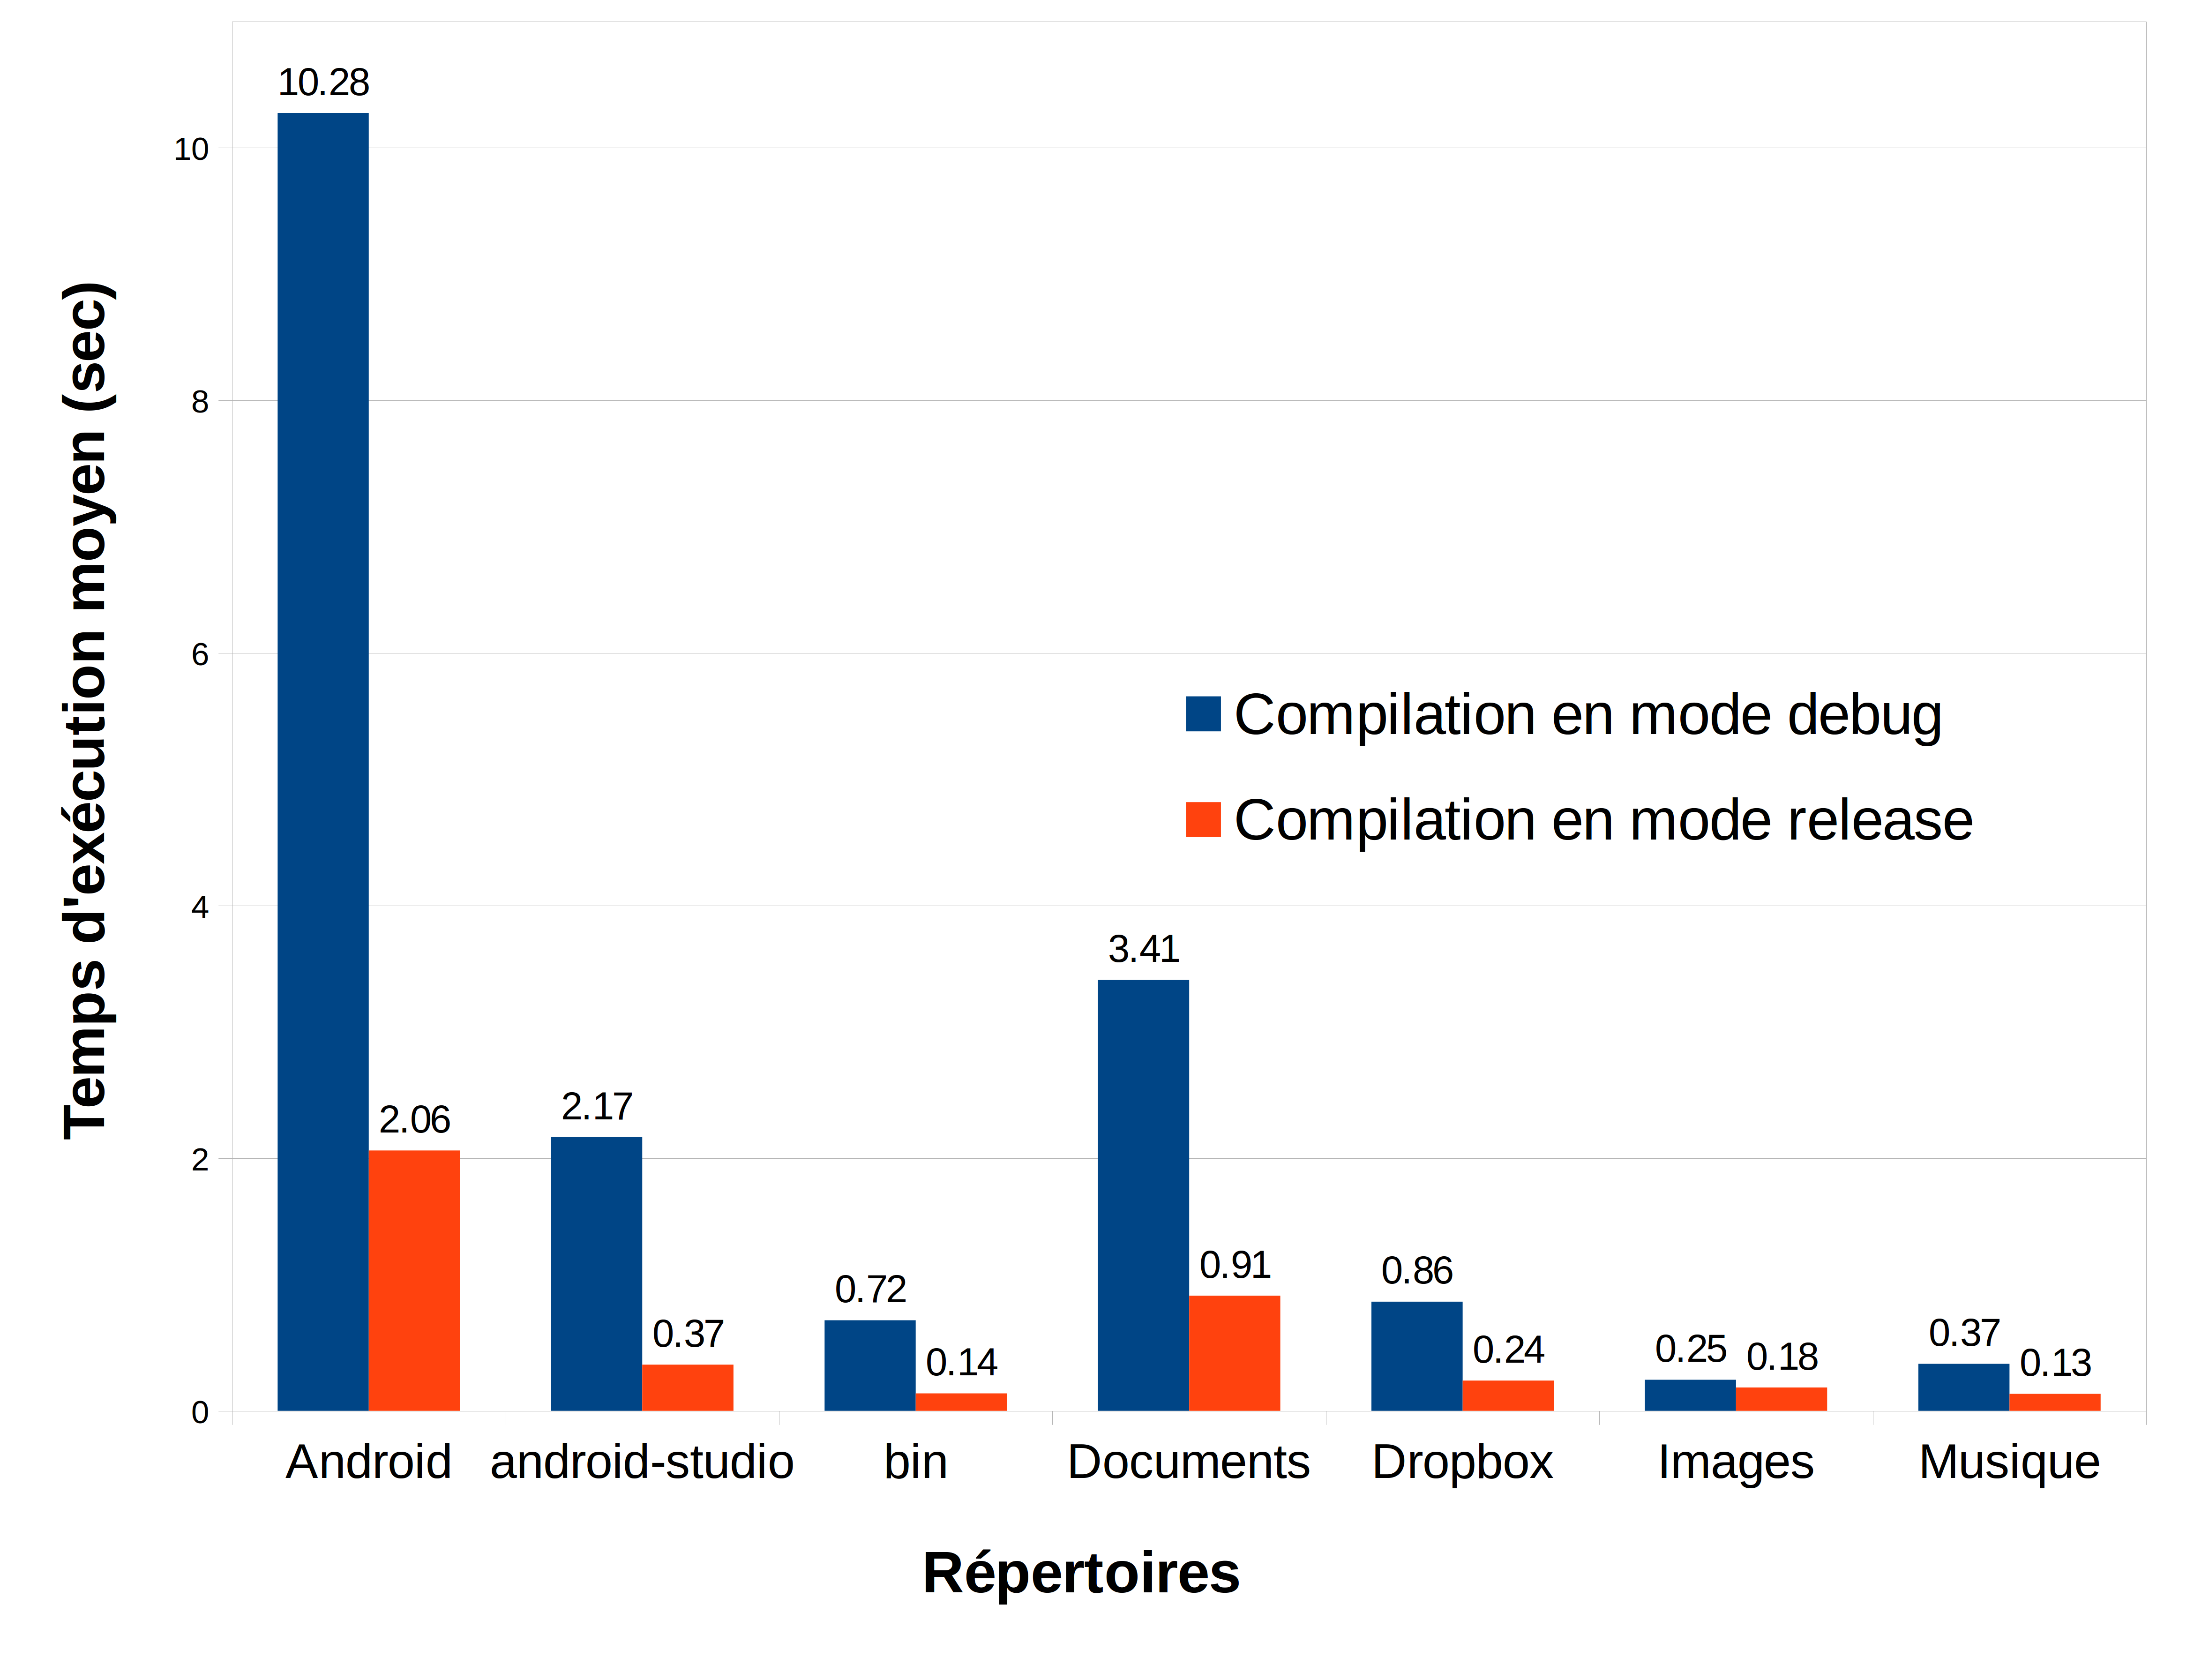
\includegraphics[width=1\textwidth]{images/histo.png}}
    \end{center}
    \caption{Temps d'exécution en fonction du répertoire}
    \label{histo}
\end{figure}
Il est intéressant de remarquer que le rapport de temps d'exécution entre la version non-optimisée 
et optimisée peut être important. La figure \ref{histo2} donne illustre ces rapports de temps. Nous 
voyons que la différence varie entre 5.93 pour \mintinline{text}{android-studio} et 1.33 pour 
\mintinline{text}{Images}, de manière générale ce sont à nouveau les répertoires 
avec le plus d'entrées qui ont les rapports les plus importants. Le répertoire \mintinline{text}{Images} 
contenant peu d'éléments en comparaison, il est difficile d'optimiser davantage le nombre 
également réduit d'opérations effectuées à l'exécution du programme. La leçon à tirer de ces rapports est 
que le compilateur Rust est capable de grandes optimisations sur le code.
\begin{figure}
    \begin{center}
        \fbox{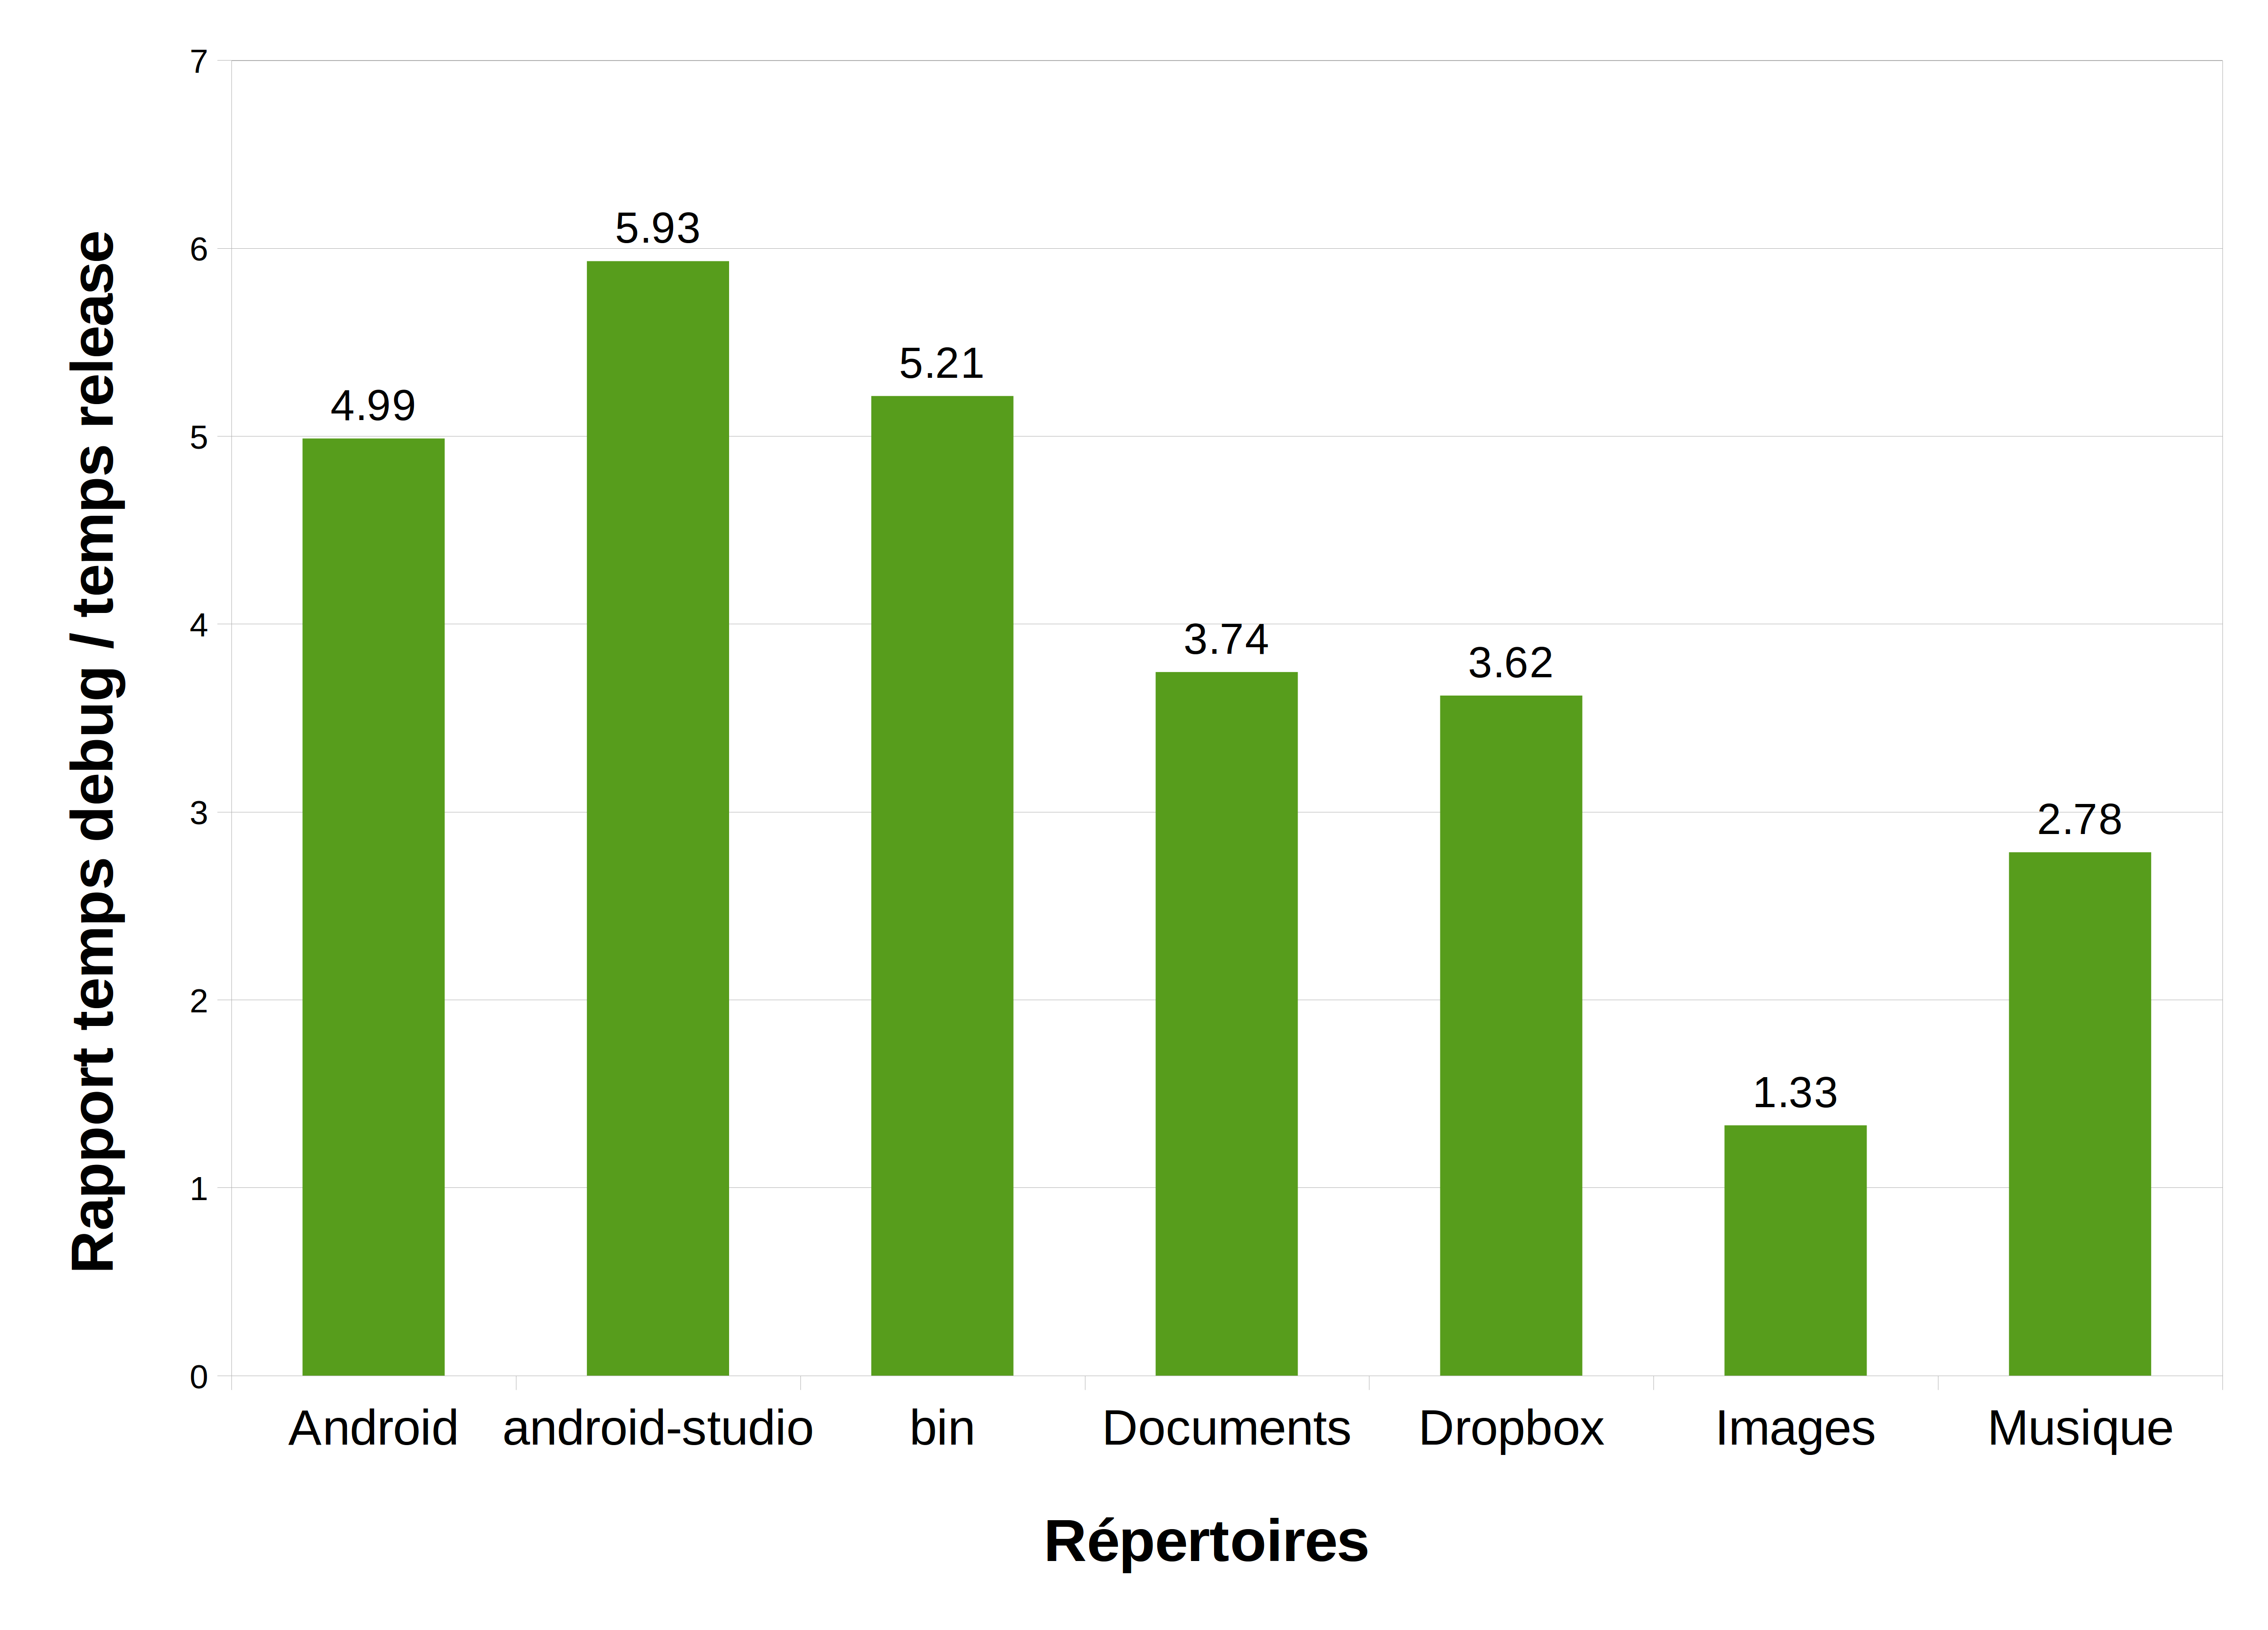
\includegraphics[width=1\textwidth]{images/histo2.png}}
    \end{center}
    \caption{Rapport entre le temps d'exécution en mode \textit{debug} et en mode \textit{release}}
    \label{histo2}
\end{figure}
%%%%%%%%%%%%%%%%%%%%%%%%%%%%%%%%%%%%%%%%%%%%%%%%%%%%%%%%%%%%%%%%%%%%%%%%%%%%%%%%%%%%%%%%%%%%%%%%%%%
%%%%%%%%%%%%%%%%%%%%%%%%%%%%%%%%%%%%%%%%%%%%%%%%%%%%%%%%%%%%%%%%%%%%%%%%%%%%%%%%%%%%%%%%%%%%%%%%%%%
\subsection{Tests unitaires avec Rust}
% TODO: tests unitaires supplémentaires
